\documentclass[11pt]{rapport-tp-qlm}
% Pour les documents écrits en général, entre 10pt et 12pt
% 11pt OBLIGATOIRE POUR LE RAPPORT de l'UE Devenir Étudiant.e

% Bonne lecture des lettres accentuées :
\usepackage[utf8]{inputenc}
% si ça ne marche pas sur des systèmes un peu anciens, à la place
% de [utf8] on peut essayer [cp1252] sur Windows, ou [latin1] sur
% Mac ou Linux / Ubuntu / Fedora

% Choix d'une police de caractères :
\usepackage{lmodern}
% Dizaines d'autres possibilités, par exemple iwona, charter... 
% Voir par exemple  http://www.tug.dk/FontCatalogue/mathfonts.html
\usepackage[T1]{fontenc} % Nécessaire avec certaines police
\usepackage[section]{placeins}
% Les paquets suivants permettent d'inclure des liens internets,
% des images, des pages pdf :
\usepackage{hyperref}
\usepackage{graphicx}
\usepackage{pdfpages}
\usepackage{listings}
\usepackage{float}
\usepackage{graphicx}
\graphicspath{ {./assets/} }
%%%%%%%  FIN DE L'EN-TÊTE - DÉBUT DU CONTENU %%%%%%
\begin{document}


\title{Rapport TP 3 - IFT3913}

\author{
	\\Loïc Daudé Mondet
	\\20243814 -- Programmes d'échanges - 1er c.(Échange)
	\\
	\\Alaa edlin Yacoub
}

\date{16/12/2022}

\maketitle

\chapter{Tests boîte noire}
\section*{Définition des tests}
On défini les classes d'équivalence comme les cas pour lesquels le programme doit se comporter à peu près de la même manière.
\subsection*{Devises}
On peut dans un premier temps tester ce qu'il se passe en faisant varier les devises. Pour ce faire on identifie les classes d'équivalence suivantes :
\begin{itemize}
  \item deux valeur dans la liste \{USD, CAD, GBP, EUR, CHF, INR, AUD\}
  \item une valeur appartient à liste et l'autre non
  \item les deux valeur n'appartiennent pas à cette liste
\end{itemize}

On peut choisir par exemple le jeu de test : 
\begin{itemize}
  \item USD, CAD
  \item USD, ZZZ
  \item XXX, ZZZ
\end{itemize}

On peut également considérer les classes où : 
\begin{itemize}
  \item une valeur n'appartient pas à la liste \{USD, CAD, GBP, EUR, CHF, INR, AUD\}, mais est quand même présente dans le fichiers json avec une valeur non valide
  \item les deux valeurs n'appartiennent pas à la liste \{USD, CAD, GBP, EUR, CHF, INR, AUD\}, mais sont quand même présentent dans le fichiers json
  \item un mélange entre une valeur dans la liste \{USD, CAD, GBP, EUR, CHF, INR, AUD\} et une autre n'appartenant à cette liste, mais présente dans le fichier json
\end{itemize}

On a alors le jeu de test suivant:
\begin{itemize}
  \item NGN, ZZZ
  \item NGN, ALL
  \item USD, NGN
\end{itemize}

Il n'y a pas de valeurs frontières car les variables sont nominales.

Normalement d'après la spécification seul le cas \{USD, CAD\} devrait renvoyer une valeur.
\newpage
\subsection*{Montants}
Pour les montant on identifie les classes suivantes : 
\begin{itemize}
  \item une valeur dans le domaine [0, 10000]
  \item une valeur en dessous de ce domaine
  \item une valeur au dessus de ce domaine
  \item une valeur frontière à la borne inférieure de ce domaine
  \item une valeur frontière à la borne supérieure de ce domaine
\end{itemize}



Ce qui donne le jeu de test suivant:
\begin{itemize}
  \item 1000
  \item -1000
  \item 11000
  \item 0
  \item 10000
\end{itemize}

On s'attend à ce que la méthode convert() renvoie la valeur correctement convertie avec les taux de change présent dans le fichier json quand la classe d'équivalence est celle dans le domaine. Idem pour les valeurs frontières. D'après la spécification elle ne doit pas accepter de valeurs en dehors du domaine, on peut donc s'attendre à une \texttt{IllegalArgumentException} quand il s'agit des classes d'équivalence correspondant aux valeurs en dehors du domaine.

\subsection*{Total}

Il y a donc 6 tests pour les devises et 5 tests pour les montants soit un total de 11 tests à effectuer.

\subsection*{Résultats}
\begin{figure}[h]
  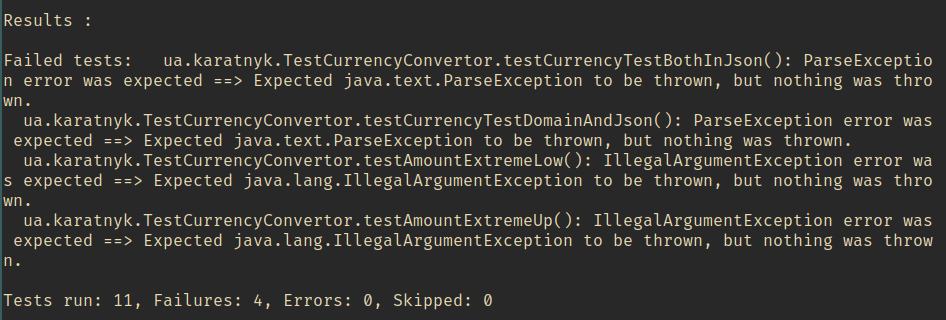
\includegraphics[scale=0.5]{assets/resbblanche}
  \centering
  \end{figure}

On remarque que 4 tests sur les 11 échouent, la méthode se comporte bien dans les plages définies par ses domaines, mais en plus elle accepte des valeurs en dehors : des devises en dehors de la liste mais dans le fichier json et des montants en dehors de l'intervalle [0,10000]. La spécification n'est donc pas respectée.
\newpage
\chapter{Tests boîte blanche}
On décide d'effectuer un critère de couverture des conditions car cela permet de trouver les erreurs les plus subtiles en évaluant au moins une fois toutes les composantes des conditions
Voici le code de \texttt{convert()}
\begin{figure}[h]
  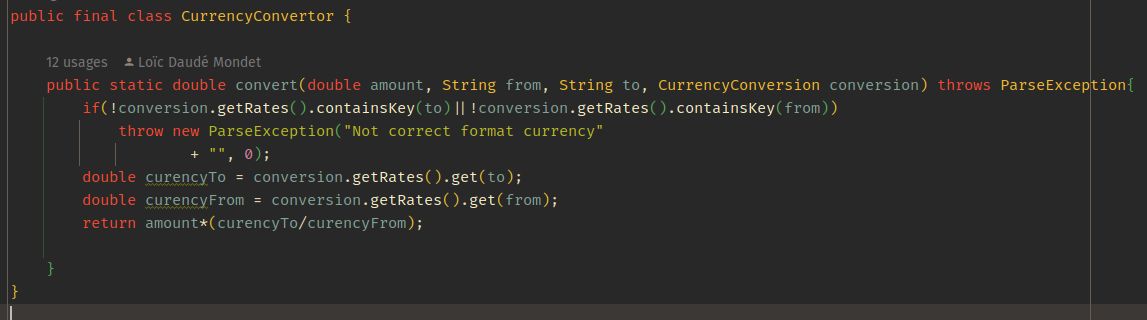
\includegraphics[scale=0.5]{assets/code}
  \centering
  \end{figure}


On identifie la condition : 

\texttt{if(!conversion.getRates().containsKey(to)||!conversion.getRates().containsKey(from))}

Il faut donc un jeu de test ou on a : 
\begin{itemize}
  \item !conversion.getRates().containsKey(to) = vrai et !conversion.getRates().containsKey(from) = vrai
  \item !conversion.getRates().containsKey(to) = vrai et !conversion.getRates().containsKey(from) = faux
  \item !conversion.getRates().containsKey(to) = faux et !conversion.getRates().containsKey(from) = vrai
  \item !conversion.getRates().containsKey(to) = faux et !conversion.getRates().containsKey(from) = faux
\end{itemize}

Les appels aux méthodes getRates et containsKey permettent de vérifier si la clef to (ou from) appartient au dictionnaire extrait du fichier json contenant les taux de conversion. Ces clefs sont les identifiants des devises comme USD ou CAD.


On se rend compte qu'on a déjà testé ces conditions lors des tests en boite blanche.

Il en ressort que si la méthode ne respecte pas la spécification demandée c'est car il manque des conditions, notamment vérifier que le montant est bien dans le domaine et que les devises à convertir appartiennent bien à notre liste réduite.



\end{document}